\begin{figure}
    \centering
    \caption{Forças internas: seção em um sólido qualquer}
    \begin{subfigure}[b]{\textwidth}
        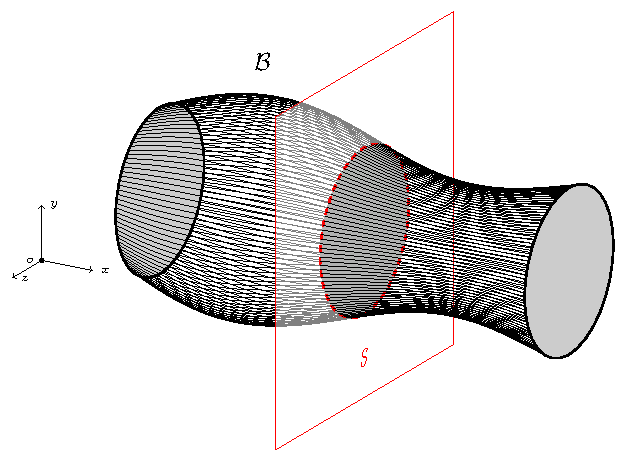
\includegraphics[scale=0.7]{Figuras/forcas_internas_2.pdf}
        \caption{$ $}
        \label{fig:forcas_internas_1}
    \end{subfigure}
    \hfill
    \begin{subfigure}[b]{\textwidth}
        \centering
        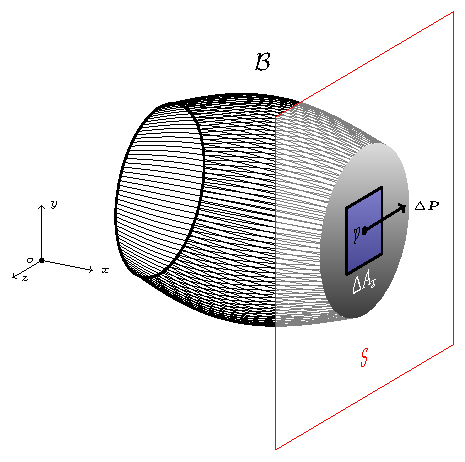
\includegraphics[scale=0.7]{Figuras/forcas_internas_1.pdf}
        \caption{$ $}
        \label{fig:forcas_internas_2}
    \end{subfigure}
    \hfill
    \begin{subfigure}[b]{\textwidth}
        \centering
        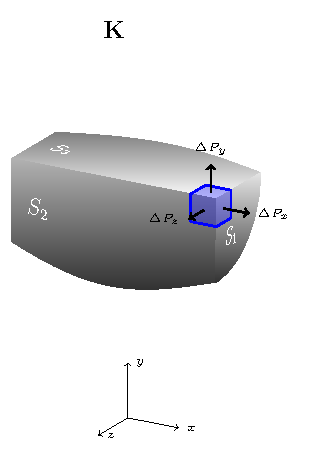
\includegraphics[scale=0.7]{Figuras/forcas_internas_3.pdf}
        \caption{$ $}
        \label{fig:forcas_internas_3}
    \end{subfigure}
       \label{fig:forcas_internas}
\end{figure}